\section{Robustness}\label{s:robust}

We now ask whether \name can effectively shift the bottleneck under a variety of conditions.

\subsection{Cross Traffic}\label{s:robust:cross}

The characteristics of other traffic --- not part of the traffic aggregate \name controls --- on the link can force \name's congestion controller to yield queue size to remain competitive in the bottleneck link.
\an{Should we say this? :}Note that under more challenging network conditions --- over-subscription, etc --- the role an importance of \name' congestion controller is more important. As we discuss in \S\ref{s:discussion}, we anticipate that future work in congestion control may yield better results.

\begin{figure}
    \centering
\begin{knitrout}
\definecolor{shadecolor}{rgb}{0.969, 0.969, 0.969}\color{fgcolor}
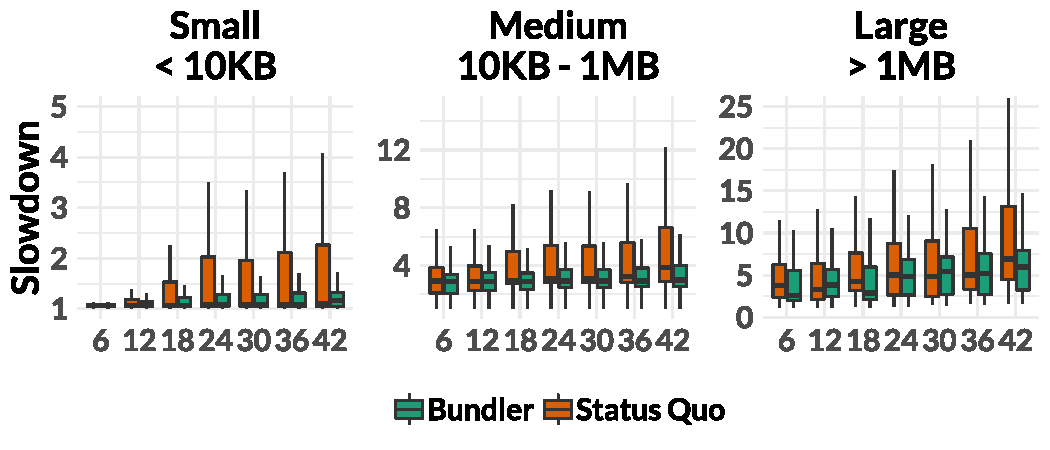
\includegraphics[width=\maxwidth]{figure/robust_cr-inelastic-1} 

\end{knitrout}
    \caption{Against cross traffic comprising of short lived flows. \name offers 48Mbps of load to the bottleneck queue. The cross traffic's offered load increases along the x-axis, while \name{}'s offered load remains fixed.}
    \label{fig:robust:cr-inelastic}
\end{figure}

\paragrapha{Inelastic Cross Traffic} We first consider the case of \emph{inelastic} cross traffic; that is, traffic that does not respond to queue-size fluctuations.
For example, traffic primarily comprised of short web requests has the inelastic property because regardless of what \name's congestion controller (or any end-to-end congestion controller) does, the component short requests, which remain in TCP slow start for their entirety, will occupy some fraction of the bottleneck link capacity.
In this case, the congestion controller must yield bandwidth to the cross traffic, but can still maintain low delays at the bottleneck link.

We can see this phenomenon in action in Figure~\ref{fig:robust:cr-inelastic}. 
Each of the congestion control algorithms we evaluate sacrifice (to varying degrees) bandwidth in reaction to the cross traffic, which hurts the FCTs of the larger requests.
However, the scheduling policy apportions the remaining bandwidth to the short flows, so there is still an improvement in FCTs at the median.

\begin{figure}
    \centering
    \begin{subfigure}[b]{0.5\textwidth}
\begin{knitrout}
\definecolor{shadecolor}{rgb}{0.969, 0.969, 0.969}\color{fgcolor}
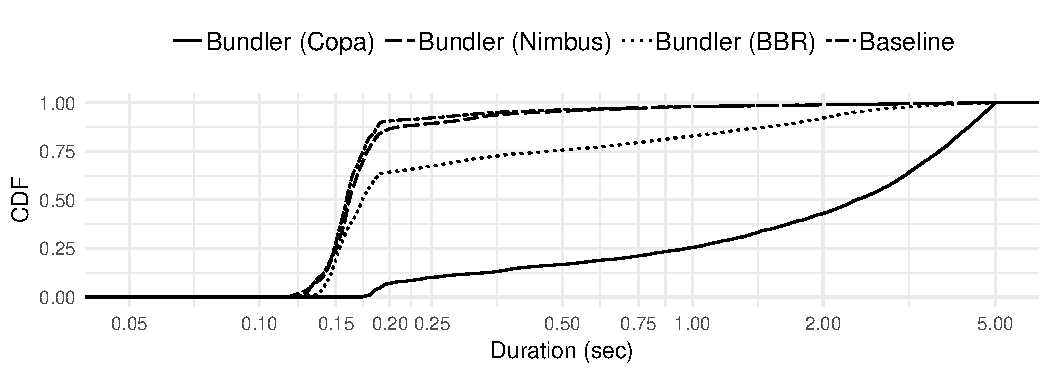
\includegraphics[width=\maxwidth]{figure/robust:cr-elastic:a-1} 

\end{knitrout}
    \caption{Congestion controllers from \S\ref{s:eval}.}\label{fig:robust:cr-elastic:a}
    \end{subfigure}
    \begin{subfigure}[b]{0.5\textwidth}
\begin{knitrout}
\definecolor{shadecolor}{rgb}{0.969, 0.969, 0.969}\color{fgcolor}
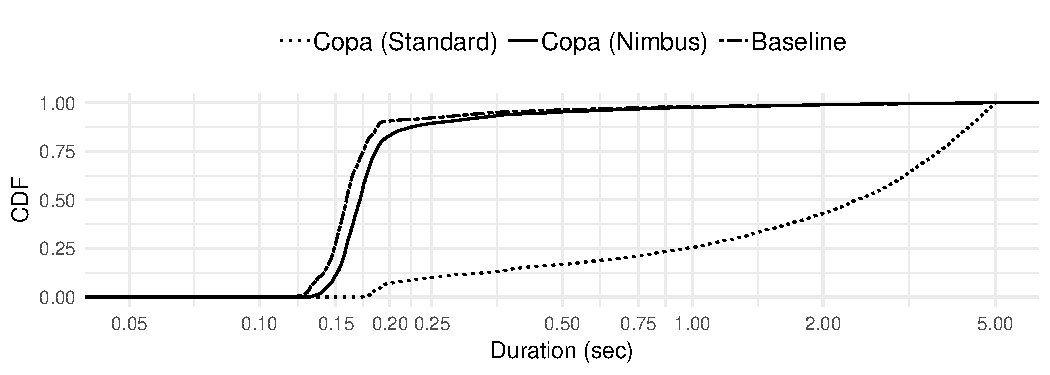
\includegraphics[width=\maxwidth]{figure/robust:cr-elastic:b-1} 

\end{knitrout}
    \caption{Alternate configuration -- Copa uses Nimbus's elasticity detector.}\label{fig:robust:cr-elastic:b}
    \end{subfigure}

    \caption{Elastic cross traffic.}
    \label{fig:robust:cr-elastic}
\end{figure}

\paragrapha{Elastic Cross Traffic} Elastic cross traffic, which fills the bottleneck link's buffer, is the worst-case scenario for \name.
The congestion controller must push packets into the bottleneck queue to compete fairly, and thus it cannot retain packets at the \inbox to schedule.
As a result, we expect performance to be no better than the baseline.
We indeed see this in Figure~\ref{fig:robust:cr-elastic}.

It is important to note that traditional loss-based congestion controllers (\ie Cubic~\cite{cubic}, NewReno~\cite{newreno}) are poor choices for \name. 
This is because they double-penalize component traffic for losses: first, in the reaction of the end-to-end congestion controller to the loss, and second in the reaction of the controller at \name.
Therefore, for algorithms which observe loss (Nimbus and Copa), we configure them to ignore it; the end-to-end reaction to loss will modulate the offered load to be the fair share of the bottleneck.

In this experiment, Copa, primarily a delay-based algorithm, cannot adequately detect the presence of competing elastic traffic and ``mode-switch'' to its competitive mode. When we modify Copa to use Nimbus's elasticity detector (Figure~\ref{fig:robust:cr-elastic:b}), its performance matches the baseline.

\begin{figure}
    \centering
\begin{knitrout}
\definecolor{shadecolor}{rgb}{0.969, 0.969, 0.969}\color{fgcolor}
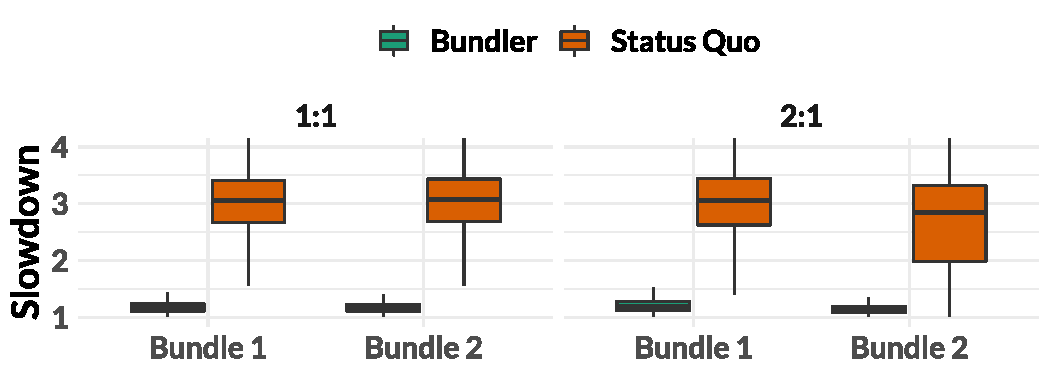
\includegraphics[width=\maxwidth]{figure/robust_twobundler-1} 

\end{knitrout}
    \caption{Competing traffic bundles. In both cases, the aggregate offered load is 84Mbps, as in Figure~\ref{fig:eval:best}. For "1:1", we evenly split the offered load between the two Bundles; for "2:1", one bundle has twice the offered load of the other. In both cases, each bundle observes improved median FCT compared to its performance in the baseline scenario.}
    \label{fig:robust:twobundler}
\end{figure}

\paragrapha{Competing Bundles} \name's improvements return once competing traffic starts using \name as well. In Figure~\ref{fig:robust:twobundler}, we show the performance of each of two bundles of traffic competing in the same bottleneck link. 
Despite both bundles containing persistently backlogged flows, just as in Figure~\ref{fig:robust:cr-elastic}, here \name improves the FCTs of both bundles independently.

\subsection{Path Characteristics}\label{s:robust:path}
\an{should these go in ``microbenchmarks'' in \S\ref{s:measurement}?}
\begin{outline}
\1 Different RTTs
\1 Different bandwidths
\end{outline}
